\section{Inference Methodology}

%For the SEI:

%Census data + geolocalization + ARPU + cellphone payments (recharges)  --> SEI estimation for geolocalized users. 

%Second, we extended our predictions taking advantage of graph structure and socioeconomic homophily. To this end, we considered a bayesian  

%\sout{As part of the dataset from the bank \( B \), we have the monthly salaries of most bank users \( B_{S_0} \cdots B_{S_t} \) for a period \( t \) larger than \( M \). We considered the average of \( B_{S_i} \) for a period of \( 6 \) moths to generate \( B_S \)}

%\sout{To infer the monthly salary of the users we take the average of \( B_{S_i} \) for a period of \( 6 \) moths to generate \( B_S \), and we compare them with other users' salaries by using the link correlations in \( G_N \).}

The main contribution of this work is the estimation of the income of the telco users for which we lack banking data but have bank clients in their neighborhood of network graph. To show the feasibility of this task we first show the existence of a strong income homophily in the telco graph as is evidenced in figure \ref{homophily_heatmap}.

For each pair \( \left< o, d \right> \in \mathlarger{G} \) we define \( X \) as the set of incomes for callers and \( Y \) as the set of incomes for callees. According to what we can observe in Figure \ref{homophily_heatmap}, \( X \) and \( Y \) should be significantly correlated. Given the broad non gaussian distribution of the income's values, which covers several different  orders of magnitude, we choose to use a rank based measure of correlation which is robust to ourliers, namely the \textbf{Spearman's rank correlation} \eqref{spearman} to test the statistical dependence of sets \( X \) and \( Y \) using the following formula:

\begin{equation}
r_s = \mathlarger{\rho}_{\operatorname{rank}(X) \operatorname{rank}(Y)} = \frac{\operatorname{cov}(\operatorname{rank}(x), \operatorname{rank}(y))}{\sigma_{\operatorname{rank}(X)} \sigma_{\operatorname{rank}(Y)}}
\label{spearman}
\end{equation}

If we compare our data with a randomized null hypothesis, where links between users are selected randomly disregarding income data, this coefficient gives us a correlation coefficient of $r_s = \mathbf{0.474} $ with a P-value of $ \mathbf{P < 10^{-6}} $. This is statistically significant enough to show that there's some amount of homophily between the users' incomes in our data.

We can take advantage of this homophily to propagate income information to the rest of our graph $ \mathlarger{P} $, where we don't know the income of all of the users.

\begin{figure}[h]
\begin{center}
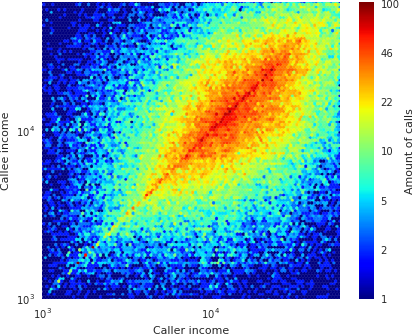
\includegraphics[width=1\columnwidth]{figures/Homophily_income_origin_target_1/Homophily_income_origin_target_1.png}
\caption{ \protectReplace this text with your caption}
\label{homophily_heatmap}
\end{center}
\end{figure}

\subsection{Prediction algorithm}

Instead of predicting the exact value of a users income, our strategy is to separate the income values into five distinct groups $ H_1, \ldots, H_5 H_5 \subseteq G$ of increasing wealth where

\[
	g \in H_i \iff g_s \in R_i
\]

where the income ranges are set as follows
\begin{align*}
	R_1 &= \left[1000, 2500\right) \\
	R_2 &= \left[2500, 7500\right) \\
	R_3 &= \left[7500, 20000\right) \\
	R_4 &= \left[20000, 50000\right) \\
	R_5 &= \left[50000, \infty\right) \\
\end{align*}

According to the Dirichlet Distibution, each user has a caller income category probability density function of the form

\[
f \left( x_1, \ldots, x_5; \alpha_1, \ldots, \alpha_5 \right) = \frac{1}{\Beta \left( \alpha \right)} \prod^5_{i = 1} x_i^{\alpha_i - 1}
\]

Where $ \Beta $ represents the Beta function,

\[
\Beta \left( \alpha_1, \ldots, \alpha_k \right) = \frac{\prod^k_{i = 1} \Gamma \! \left( \alpha_i \right)}{\Gamma \! \left( \sum^k_{i = 1} \alpha_i \right) }
\]

For all the other users in the telco having at least one link to any other telco user with a defined income $ q \in Q = \left\{x \in \left( N \setminus B \right) \mid (\exists y \in G) \left< x, y \right> \in P \vee \left< y, x \right> \in P \right\} $, we can use this distribution to infer the probabilities of being part of each group $ H_1, \ldots, H_5 $, and this way approximate the economic status.
